\newpage
\section{Relation Model}

A \hl{relational database} is a collection of one or more \hl{relations}, which are based on the relational model. A \hl{relation} is a \hl{table} with \hl{rows} and \hl{columns}. The major advantages of the relational model are its \hl{straightforward data representation} and \hl{the ease} with which even complex queries can be expressed. 

relationship and relation
\begin{itemize}
    \item A \hl{relationship} is an association among several \hl{entities}.
    \item A \hl{relation} is the mathematical concept, referred to as a \hl{table}. 
\end{itemize}

\subsection{Structure of Relational Databases}
\subsubsection{Basic Structure}
Formally, given sets $D_1,D_2,\dots,D_n (D_i=a_{ij}|_{j=1,\dots,k})$, a relation $r$ is a subset of $D_1\times D_2\times \dots \times D_n$ --- a \hl{Cartesian product} of a list of domain $D_i$. Thus a relation is a set of n-tuples $(a_{1j},a_{2j},\dots,a_{nj})$, where each $a_{ij}\in D_i (i\in [1,n]) $. 

\subsubsection{Attribute Types}
Each attribute of a relation has a name. The set of allowed values for each attribute is called the \hl{domain} of the attribute. Attribute values are (normally) required to be \hl{atomic}, i.e., \hl{indivisible}. (--- 1st NF, 关系理论第一范式). The special value \hl{null} is a member of every domain. The \hl{null} value causes complications in the definition of many operations.

\subsubsection{Concepts about Relation}
A relation is concerned with two concepts: relation schema and relation instance.
\begin{itemize}
    \item The \hl{relation schema} describes the structure of the relation.
    \item The \hl{relation instance} corresponds to the \hl{snapshot} of the data in the relation at a given instant in time.
\end{itemize}

\subsubsection{Relation Schema}
Assume $A_1,A_2,\dots,A_n$ are attributes. Formally expressed: $R=(A_1,A_2,\dots,A_n)$ is a relation schema. $r(R)$ is a relation on the relation schema $R$. 

\subsubsection{Relation Instance}
The current values (i.e., relation instance) of a relation are specified by a table. An element $t$ of $r$ is a tuple, represented by a row in a table. 

Let a tuple variable $t$ be a tuple, then t[name] denotes the value of $t$ on the name attribute.

\subsubsection{The Properties of Relation}
\begin{enumerate}
    \item The order of tuples is irrelevant. 
    \item No duplicated tuples in a relation.
    \item Attribute values are atomic.
\end{enumerate}

\subsubsection{Database}
A database consists of multiple relations. Information about an enterprise (e.g., university) is broken up into parts. 

Normalization theory (Chapter 7) deals with how to design ``good'' relational schemas. 


\subsubsection{Key (码/键)}
Let $K \subseteq R$. 
\begin{enumerate}
    \item K is a \hl{superkey (超码)} of R if values for K are \hl{sufficient} to identify a unique tuple of each possible relation r(R). 
    \item K is a \hl{candidate key (候选码)} if K is \hl{minimal superkey}.
    \item K is a \hl{primary key (主码)}, if K is a candidate key and is \hl{defined by user explicitly}. Primary key is usually \hl{marked by underline}. 
\end{enumerate}

\subsubsection{Foreign Key (外键/外码)}
Assume there exists relations $r$ and $s$: $r(\underline{A}, B, C)$, $s(\underline{B}, D)$, we can say that attribute $B$ in relation $r$ is foreign key referencing $s$, and $r$ is a \hl{referencing relation (参照关系)}, and s is a \hl{referenced relation (被参照关系)}. 

Primary key and foreign key are \hl{integrated constraints}.

\subsubsection{Schema Diagram}
\begin{figure}[H]
    \centering
    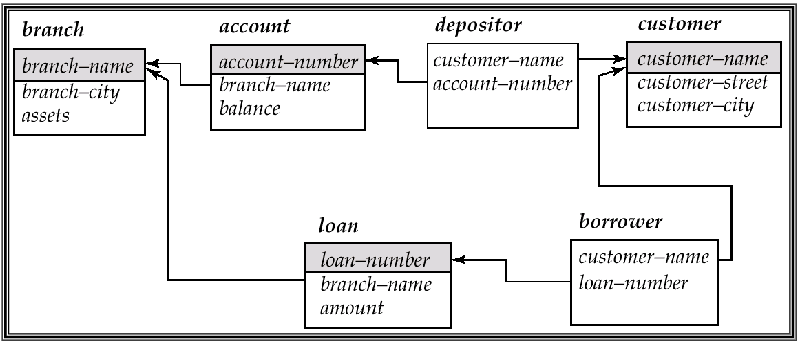
\includegraphics[width=0.209\textwidth]{DB2/Schema Diagram}
    \caption{Schema Diagram}
\end{figure}

\subsubsection{Query Languages}
Relational Algebra

\subsection[Fundamental Relational-Algebra Operations]{Fundamental Relational-Algebra Operat-ions}

\begin{enumerate}
    \item Select 选择
    \item Project 投影
    \item Union 并
    \item set difference 差(集合差)
    \item Cartesian product 笛卡儿积
    \item Rename 改名(重命名)
\end{enumerate}
The operators take one or two relations as inputs, and return a new relation as a result. 

\subsubsection{Select Operation Formalization}
Notation: $\sigma_p(r)$, $p$ is called the selection predicate. Defined as: 
\begin{align*}
    \sigma_p(r)=\left\{ t|\, t\in r\text{ and }p(t) \right\}
\end{align*}
where $p$ is a formula in propositional calculus consisting of terms connected by $\land, \lor , \lnot $. Each term is one of
\begin{align*}
    <attribute> op <attribute> or <constant>
\end{align*}
where op is one of $=, \ne, >, \ge, <, \le$. 



\subsubsection{Project Operation Formalization}
Notation: $\prod_{A_1,A_2,\dots,A_k} (r)$, where $A_1,A_2,\dots,A_k$ are attribute names and $r$ is a relation name. The result is defined as the relation of k columns obtained by erasing the columns that are not listed. Duplicate rows removed from result, since relations are sets.

\subsubsection{Union Operation Formalization}
Notation: $r \cup s$. Defined as: 
\begin{align*}
    r \cup s = \left\{ t| \, t\in r\text{ ot }t \in s \right\}
\end{align*} 

For $r\cup s$ to be valid: 
\begin{itemize}
    \item $r$ and $s$ must have the same arity. (i.e., the same number of attributes)
    \item The attribute domains must be compatible. 
\end{itemize}

\subsubsection{Set Difference Operation Formalization}
Notation: $r-s$. Defined as 
\begin{align*}
    r-s=\left\{ t| \, t \in r\text{ and }t\notin s \right\}
\end{align*}

Set differences must be taken between compatible relations.
\begin{itemize}
    \item $r$ and $s$ must have the same arity.
    \item Attribute domains of $r$ and $s$ must be compatible.
\end{itemize}

\subsubsection[Cartesian-Product Operation Form-alization]{Cartesian-Product Operation Formalization}
Notation: $r\times s$. Defined as: 
\begin{align*}
    r\times s =\left\{ \left\{ t\, q \right\}|\, t \in r\text{ and }q \in s \right\}
\end{align*}
Assume that attributes of $r(R)$ and $s(S)$ are disjoint (i.e., $R \cap S = \emptyset$). If attributes of $r(R)$ and $s(S)$ are not disjoint, then renaming for attributes must be used.

\subsubsection{Composition of Operations}
Can build expressions using multiple operations.

\subsubsection{Rename Operation}
Allows us to name, and therefore to refer to, the results of relational-algebra expressions. (procedural). Allows us to refer to a relation by more than one name.

E.g. 
\begin{align*}
    \rho_X (E)
\end{align*}
returns the expression $E$ under the name $X$. 

If a relational-algebra expression $E$ has arity $n$, then
\begin{align*}
    \rho_{X(A_1,A_2,\dots,A_n)} (E)
\end{align*}
returns the result of expression $E$ (对relation E及其attributes都重命名). 

\subsection{Additional Relational-Algebra Operations}
\begin{enumerate}
    \item Set intersection 交
    \item Natural join 自然连接
    \item Division 除
    \item Assignment 赋值
\end{enumerate}
We define additional operations that do not add any power to the relational algebra, but that simplify common queries.

\subsubsection{Set-Intersection Operation Formalization}
Notation: $r\cap s$. Defined as: 
\begin{align*}
    r \cap s=\left\{ t | \, t \in r\text{ and }t \in s  \right\}
\end{align*}

Assume: 
\begin{itemize}
    \item r and s have the same arity.
    \item attributes of r and s are compatible. 
\end{itemize}

Note: $r\cap s = r - (r-s)$.  

\subsubsection{Natural Join Operation Formalization}
Notation: $r \bowtie  s$. 

e.g. R = (A, B, C, D), S = (B, D, E)
\begin{itemize}
    \item Result schema of the natural-join of r and s = (A, B, C, D, E)
    \item $\displaystyle r \bowtie s = \prod_{r.A, r.B, r.C, r.D, s.E} (\sigma_{r.B=s.B \land r.D = s.D}(r\times s))$
\end{itemize}

Let $r$ and $s$ be relations on schemas $R$ and $S$, respectively. Then, $r \bowtie s$ is a relation on schema $R \cup S$ obtained as follows: Consider each pair of tuples $t_r$ from $r$ and $t_s$ from $s$. If $t_r$ and $t_s$ have the same value on each of the attributes in $R \cap S$, add a tuple $t$ to the result, where
\begin{itemize}
    \item $t$ has the same value as $t_r$ on $r$. 
    \item $t$ has the same value as $t_s$ on $s$. 
\end{itemize}

\subsubsection{Division Operation Formalization}
Notation: $r\div s$. Let $r$ and $s$ be relations on schemas $R$ and $S$, respectively, where $R = (A_1, \dots, A_m, B_1, \dots, B_n)$ and $S = (B_1, \dots, B_n)$. Then, the result of $r \div s$ is a relation on the schema $R – S = (A_1, \dots, A_m)$ and
\begin{align*}
    r\div s=\left\{ t \left| \, t \in \prod_{R-S}(r) \land \forall u \in s(tu \in r )\right. \right\}
\end{align*}

Note that $\prod_{R-S}(r)$ encloses the result of $r \div s$, and meanwhile, the  union of the tuple(s) $t$ and all the tuples in $s$ is covered by $r$ (i.e., 商来 自于$\prod_{R-S}(r)$, 并且其元组$t$与$s$所有元组的拼接被$r$覆盖).

Division Operation Characteristic: Let $q = r \div s$, then $q$ is the largest relation satisfying $q \times s \subseteq r$. 

\subsubsection{Assignment Operation}
The assignment operation $(\leftarrow)$ provides a convenient way to
express complex queries.
\begin{enumerate}
    \item Write query as a sequential program consisting of
    \begin{itemize}
        \item A series of assignments.
        \item Followed by an expression whose value is displayed as a result of the query.
    \end{itemize}
    \item Assignment must always be made to a temporary relation variable.
\end{enumerate}

e.g. Write $r\div s $ as:
\begin{align*}
    temp1 \leftarrow& \prod_{R-S}(r)\\
    temp2 \leftarrow& \prod_{R-S}\left((temp1\times s)-\prod_{R-S}(r)\right)\\
    result=& temp1-temp2
\end{align*}

\subsubsection{Summary}
\begin{itemize}
    \item Union, set difference, Set intersection 为双目、等元运算
    \item Cartesian product, Natural join, Division 为双目运算
    \item Project, select 为单运算对象 (i.e., 单目运算)
\end{itemize}

The priority of operations is as follows:
\begin{enumerate}
    \item Project
    \item Select
    \item Cartesian Product (times)
    \item Join, division
    \item Intersection
    \item Union, difference
\end{enumerate}

\subsection{Extended Relational-Algebra Operations}
\begin{enumerate}
    \item Generalized Projection 泛化投影
    \item Aggregate Functions 聚合处理
    \item Outer Join 外链接
\end{enumerate}

\subsubsection{Generalized Projection}
Extends the projection operation by allowing arithmetic functions to be used in the projection list.
\begin{align*}
    \prod_{F_1,F_2,\dots,F_n}(E)
\end{align*}
where $E$ is any relational-algebra expression, and each of $F_1,F_2,\dots,F_n$ are arithmetic expressions involving constants and attributes in
the schema of $E$.

\subsubsection{Aggregate Functions and Operations}
Aggregation function takes a collection of values and returns a single value as a result.
\begin{itemize}
    \item avg: average value
    \item min: minimum value
    \item max: maximum value
    \item sum: sum of values
    \item count: number of values
\end{itemize}

Aggregate operation in relational algebra
\begin{align*}
    {}_{G_1,G_2,\dots,G_n}g_{F_1(A_1),F_2(A_2),\dots,F_n(A_n)}(E)
\end{align*}
where $E$ is any relational-algebra expression, $G_1,\dots,G_n$ is a list of attributes on which to group (can be empty), each $F_i$ is an aggregate function, and each $A_i$ is an attribute name.

Result of aggregation does not have a name. For convenience, we permit renaming as part of aggregate operation. 

\begin{align*}
    {}_A g_{sum(C) \text{ as abc}}(r)
\end{align*}

\subsubsection{Outer Join}

An extension of the join operation that avoids loss of information. Computes the join and then adds tuples form one relation that does not match tuples in the other relation to the result of the join. Uses null values:
\begin{enumerate}
    \item null signifies that the value is unknown or does not exist. 
    \item All comparisons involving null are false by definition (roughly speaking). We shall study precise meaning of comparisons with nulls later. 
\end{enumerate}

$\sqsupset\hspace*{-2pt}\bowtie\hspace*{-2pt}\sqsubset$

\subsubsection{Null Values}
The result of any arithmetic expression involving null is null. 

Aggregate functions simply ignore null values.  

For duplicate elimination and grouping, null is treated like any other value, and two nulls are assumed to be the same. 

Comparisons with null values return the special truth value:
unknown.  Three-valued logic using the truth value unknown:
\begin{itemize}
    \item OR: 
    \begin{itemize}
        \item (unknown or true) = true,
        \item (unknown or false) = unknown
        \item (unknown or unknown) = unknown 
    \end{itemize}
    \item AND: 
    \begin{itemize}
        \item (true and unknown) = unknown,
        \item (false and unknown) = false,
        \item (unknown and unknown) = unknown
    \end{itemize}
    \item NOT: (not unknown) = unknown
    \item In SQL “P is unknown” evaluates to true if predicate P evaluates to unknown. 
\end{itemize}
Result of select predicate is treated as false if it evaluates to unknown. 

\subsection{Modification of the Database}
The content of the database may be modified using the following operations:
\begin{enumerate}
    \item Deletion
    \item Insertion
    \item Updating
\end{enumerate}
All these operations are expressed using the assignment operator.

\subsubsection{Deletion}

A deletion is expressed in relational algebra by:
\begin{align*}
    r \leftarrow r - E
\end{align*}
where $r$ is a relation and $E$ is a relational algebra query.

\subsubsection{Insertion}
In relational algebra, an insertion is expressed by:
\begin{align*}
    r \leftarrow r \cup E
\end{align*}
where $r$ is a relation and $E$ is a relational algebra expression.

\subsubsection{Update}
Use the generalized projection operator to do this task
\begin{align*}
    r \leftarrow \prod_{F_1,F_2,\dots,F_n} (r)
\end{align*}
where each $F_i$ is either the i-th attribute of $r$, if the i-th attribute is not updated, or, if the attribute is to be updated $F_i$ is an expression, involving only constants and the attributes of $r$, which gives the new value for the attribute.

% Exercises: 2.12, 2.14, and 2.15 (see Page 62)